\chapter{Prototyping Platforms}
\label{chp:prototyping-platform}

Our file system metadata policy engines are built on top of
Malacology~\cite{sevilla:eurosys17-malacology}, which is a programmable storage
system we prototyped on Ceph~\cite{weil:osdi2006-ceph}.

\section{Ceph: A Distributed Storage System}

Ceph is a distributed storage platform that stripes and replicates data across
a reliable object store, called RADOS~\cite{weil_rados_2007}. Clients talk
directly to object storage daemons (OSDs) on individual disks. This is done by
calculating the data's placement (``where should I store my data") and location
(``where did I store my data") using a hash-based algorithm called
CRUSH~\cite{weil_crush_2006}. Ceph leverages all resources in the cluster by
having OSDs work together to load balance data across disks.

CephFS is the POSIX-compliant file system that uses RADOS. CephFS is an
important part of the storage ecosystem because it acts as a file gateway for
legacy applications. It decouples metadata and data access, so data IO is done
directly with RADOS while all metadata operations go to a separate metadata
cluster. This metadata cluster exposes a hierarchical namespace to the user
using a technique called dynamic subtree
partitioning~\cite{weil:sc2004-dyn-metadata}. In this scheme, each metadata
server (MDS) manages a subtree in the namespace. The MDS cluster is connected
to the clients to service metadata operations and to RADOS so it can
periodically flush its state. The CephFS components, including RADOS, the MDS
cluster, and the logical namespace, are shown Figure~\ref{ceph-arch}. 

\begin{figure*}[t]
\centering
	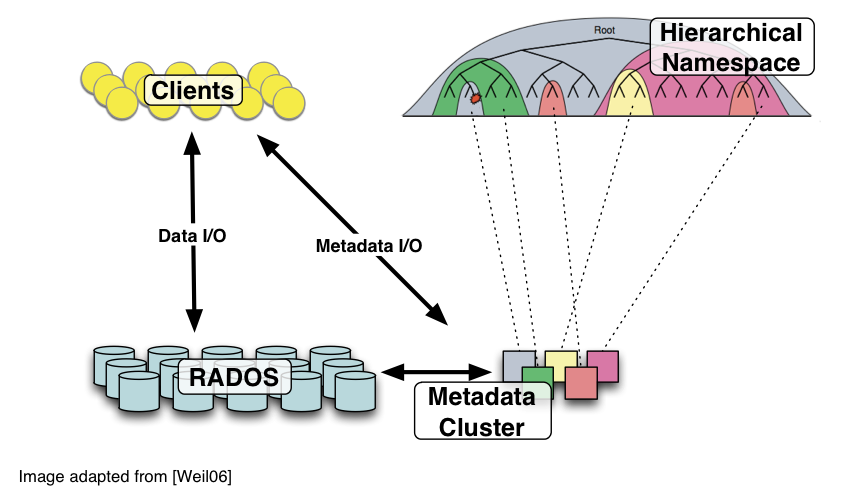
\includegraphics[width=0.7\textwidth]{./chapters/advancement/figures/ceph-arch.png} 

	\caption{In CephFS, the clients interact with a metadata server (MDS)
        cluster for all metadata operations. The MDS cluster exposes a hierarchical
        namespace using a technique called dynamic subtree partitioning, where each MDS
        manages a subtree in the namespace.\label{ceph-arch}}

\end{figure*}

\subsection*{Why Use CephFS?}
\label{background-why}

CephFS has one of the most advanced metadata infrastructures and we use it as a
prototyping platform because the file system metadata management mechanisms,
such as migration, monitoring, and journaling, are already implemented.  For
example, when many creates or writes are made in the same directory, the file
metadata can be hashed across multiple metadata servers. When many reads or
opens are made to the same file, the contents can be replicated across
different metadata servers. CephFS also other infrastructure already in-place,
such as: 

\begin{itemize}

\item ``\textbf{soft state}" for locating metadata: each MDS is only aware of
the metadata in its own cache so clients are redirected around the MDS cluster
and maintain their own hierarchical boundaries; distributed cache constraints
allow path traversal to start at any node and to be redirected upon
encountering a subtree bound.

\item \textbf{locking} to maintain consistency: replicas are read-only and all
updates are forwarded to the authority for serialization/journaling; each
metadata field is protected by a distributed state machine.

\item \textbf{counters} to identify popularity: each inode and directory
fragment maintains a popularity vector to aid in load balancing; MDSs share
their measured loads so that they can determine how much to offload and who to
offload to.

\item ``\textbf{frag trees}" for large directories: interior vertices split by
powers of two and directory fragments are stored as separate objects

\item ``\textbf{traffic control}" for flash crowds (i.e.  simultaneous
clients): MDSs tell clients if metadata is replicated or not so that clients
have the choice of either contacting the authority MDS or replicas on other
MDSs.

\item ``\textbf{migration}" for moving a subtree's cached metadata; performed
as a two-phase commit: the importing MDS journals metadata (Import event), the
exporting MDS logs the event (Export event), and the importing MDS journals the
event (ImportFinish). 

\end{itemize}

Another reason for choosing Ceph and CephFS is that the software is open-source
under the GNU license. It is also backed by a vibrant group of developers and
supported by a large group of users.
